\chapter{Introducción específica} % Main chapter title

\label{Chapter2}

%----------------------------------------------------------------------------------------
%	SECTION 2 resume 
%----------------------------------------------------------------------------------------
Se presentan las bases matemáticas del control de actitud. El control de actitud se basa en seleccionar al menos dos sistemas de referencia para definir las orientaciones a través de una matriz. Al seleccionarse dos referencias puede utilizarse diferentes parametrizaciónes de la matriz: 
\begin{itemize}
	\item Quaterniones
	\item Parámetros de Rodrigues
	\item etc... 
\end{itemize}
Estas parametrizaciones presenta ventajas sobre la matriz. La idea central del control de actitud es estimar la matriz de orientaciones En este contexto la matriz se conoce como "matriz de Actitud" (o en inglés attitude) \citep{ARTICLE:1}. 
%Esta matriz se obtiene a partir de la parametrización y del modelo dinámico del sistema, donde lo que se obtiene es una estimación y no la matriz real, según el algoritmo utilizado. 
 
 
 
 

\section{Bases ortonormales, Coordenadas y Matriz de actitud}
\label{sec:matriz_actitud}
En el espacio tridimensional, consideramos dos sistemas de referencia, uno se denomina $\mathbf{N}$ y el otro $\mathbf{B}$. Cada una de estas bases  la denotamos así: 
\begin{equation}
	\mathbf{N} = \{ \hat{n}_1, \hat{n}_2, \hat{n}_3 \}
	\qquad
	\mathbf{B} = \{ \hat{b}_1, \hat{b}_2, \hat{b}_3 \}
\end{equation}
Cada una de las bases posee las siguientes propiedades: 

\begin{itemize}
\item Los vectores $\hat{n}_i$ y $\hat{b}_i$, para $i = 1, 2, 3$, son ortogonales entre sí.
\item Los vectores $\hat{n}_i$ y $\hat{b}_i$ son unitarios.
\item Las bases $\mathbf{N}$ y $\mathbf{B}$ respetan la regla de la mano derecha: 
$\hat{b}_1 \times \hat{b}_2 = \hat{b}_3$ y $\hat{n}_1 \times \hat{n}_2 = \hat{n}_3$.
\end{itemize}


Dado un vector cualquiera $\vec{x}$ en el espacio tridimensional, es posible expresar dicho vector en términos de diferentes bases. En particular, se consideran las bases $\mathbf{N} = \{\hat{n}_1, \hat{n}_2, \hat{n}_3\}$ y $\mathbf{B} = \{\hat{b}_1, \hat{b}_2, \hat{b}_3\}$, se puede escribir el vector $\vec{x}$ como una combinación lineal de los vectores de cualquiera de estas bases. Por ejemplo, respecto de la base $\mathbf{N}$, el vector se expresa como:
\begin{equation}
	^N\vec{x} = x_1^N \hat{n}_1 + x_2^N \hat{n}_2 + x_3^N \hat{n}_3
\end{equation}

Y respecto de la base $\mathbf{B}$, se escribe como:
\begin{equation}
	^B\vec{x} = x_1^B \hat{b}_1 + x_2^B \hat{b}_2 + x_3^B \hat{b}_3
\end{equation}
Los escalares $x_1^N, x_2^N, x_3^N$ se denominan las \textbf{coordenadas del vector $\vec{x}$ en la base $\mathbf{N}$}, mientras que $x_1^B, x_2^B, x_3^B$ son sus \textbf{coordenadas en la base $\mathbf{B}$}. Aunque el vector $\vec{x}$ representa la misma entidad geométrica en ambos casos, su expresión depende de la base utilizada.

Para expresar el vector $^N\vec{x}$ en la base  $\mathbf{B}$ y viceversa se lo realiza mediante una matriz de $3 \times 3$ conocida como matriz de cosenos directores: 
\begin{equation}
	\begin{bmatrix}
		x_1^B \\
		x_2^B \\
		x_3^B
	\end{bmatrix}
	= \mathbf{M} {^A\vec{x}} = 
	\begin{bmatrix}
		\hat{b}_1 \cdot \hat{n}_1  & \hat{b}_1 \cdot \hat{n}_2  &  \hat{b}_1 \cdot \hat{n}_3  \\
		\hat{b}_2 \cdot \hat{n}_1  & \hat{b}_2 \cdot \hat{n}_2  &  \hat{b}_2 \cdot \hat{n}_3 \\
		\hat{b}_3 \cdot \hat{n}_1  & \hat{b}_3 \cdot \hat{n}_2  & \hat{b}_3 \cdot \hat{n}_3  
	\end{bmatrix}
	\begin{bmatrix}
		x_1^A \\
		x_2^A \\
		x_3^A
	\end{bmatrix}
\end{equation}

La matriz denominada  $\mathbf{M}$ es la \textbf{matriz de Actitud}. Es una matriz ortogonal. Las matrices ortogonales tienen las siguientes propiedades: 

\begin{itemize}
	\item $\mathbf{M}^T = \mathbf{M}^{-1}$
	\item $\det( \mathbf{M}) = \pm 1$ 
\end{itemize}
Sin embargo, en el contexto de rotaciones físicas en el espacio tridimensional, solo se consideran aquellas matrices ortogonales cuya determinante es igual a 1. Estas matrices forman el grupo especial ortogonal, denotado como $SO(3)$. 

\subsection{Rotaciones activas vs Pasivas}
La sección anterior denota un vector $\vec{x}$ abstracto fijo,  cuya representación cambia al modificar el sistema de referencia. Esta perspectiva se conoce como interpretación \textit{pasiva}\footnote{A veces se la conoce como Alias}. Alternativamente ,puede optarse por una interpretación  \textit{activa}\footnote{Conocida tambien como Alibi}, 
en la que el vector $\vec{x}$ es rotado a un nuevo vector $\vec{x}'$. Ambas interpretaciones conducen al mismo resultado numérico pero el significado físico es distinto. Esta diferencia de interpretación se observa en la figura \ref{fig:cmp_act_vs_rot} que compara ambas interpretaciones. 

Puede observarse en la figura \ref{fig:cmp_act_vs_rot} que compara los dos tipos de  rotaciones. En el caso de la figura \ref{fig:rotPas} el vector $\vec{x}$ tiene coordenadas $x_1,x_2$ en el sistema $\textbf{N}$ y $x'_1,x'_2$ en el sistema $\textbf{B}$, donde el sistema de referencia $\textbf{B}$  posee una rotación de ángulo $\theta$ respecto de $\textbf{N}$.  En cambio, en la figura \ref{fig:rotAct}, correspondiente a la rotación activa, el sistema de referencia $\textbf{N}$ permanece fijo, y el vector $\vec{x}$ rota un ángulo $\theta$ hasta convertirse en $\vec{x}'$.

La diferencia clave está en la dirección de la rotación: es opuesta en ambos casos, por lo que los ángulos tienen signos contrarios. Sin embargo, las coordenadas resultantes ${x'_1, x'_2}$ son idénticas en valor numérico. En este contexto, se trabajará utilizando la \textbf{interpretación pasiva} de las rotaciones.



\begin{figure}[!htpb]

	\begin{subfigure}[b]{0.49\linewidth}
%		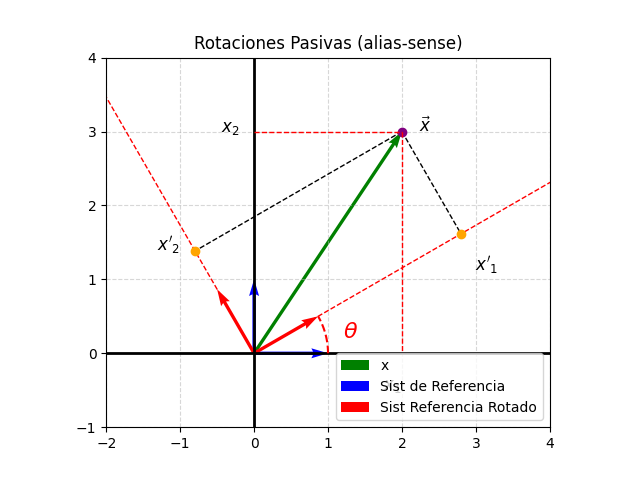
\includegraphics[scale=0.65]{./Figures/PasiveRot.png}
		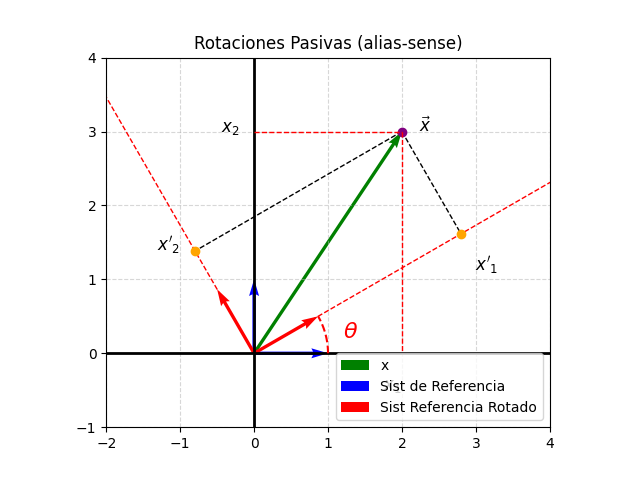
\includegraphics[width=\linewidth,height=0.25\textheight]{./Figures/PasiveRot.png}

		\caption{Rotacion Pasiva o Alias}
		\label{fig:rotPas}
	\end{subfigure}
	\hfill
	\begin{subfigure}[b]{0.49\linewidth}
%		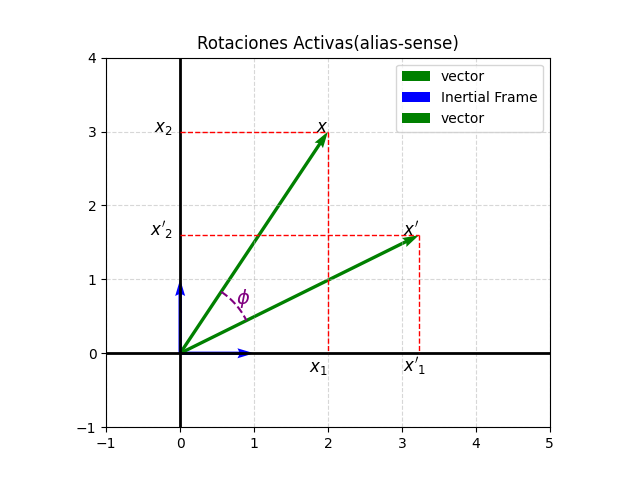
\includegraphics[scale=0.65]{./Figures/ActiveRot.png}
		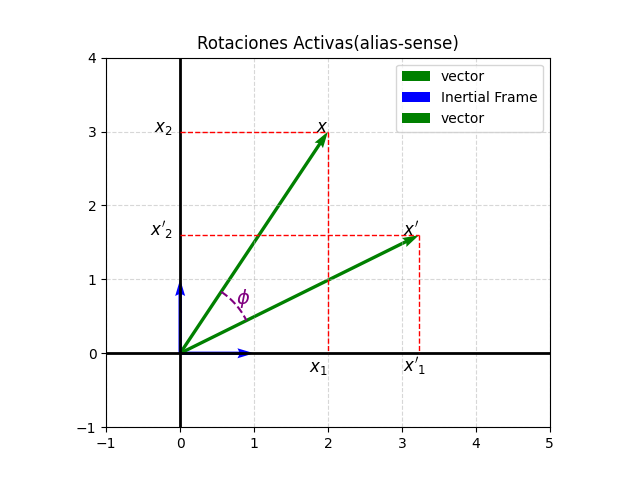
\includegraphics[width=\linewidth, height=0.25\textheight]{./Figures/ActiveRot.png}

		\caption{Rotacion Activa o alibi}
		\label{fig:rotAct}
	\end{subfigure}
	\caption{Rotacion activa y pasiva.}
	\label{fig:cmp_act_vs_rot}
\end{figure}

\subsection{Teorema de Euler}
El control de actitud es una disciplina que se encarga del estudio de las matrices de rotación ortogonales que transforman las coordenadas de un vector de un sistema de referencia a otro. 

El teorema de Euler asegura que cualquier rotación es una rotación alrededor de un eje fijo. Este eje se denota como $\vec{e}$ y es un vector unitario y la rotación de un ángulo $\vartheta$. A partir de ahora las matriz de actitud la denotamos como $\textbf{A}$. Esto implica que el vector $\vec{e}$ tiene la misma representación en coordenadas de un sistema de referencia o en otro. En terminos matemáticos implica que $\vec{e}$ es el autovector del autovalor 1 de la matriz de actitud. Este teorema da lugar a a que si se conoce el vector $\vec{e}$ y el angulo de rotación $\vartheta$ puede armarse la matriz de actitud \textbf{A} como sigue\footnote{Formula de Rodriguez}: 
\begin{equation}\label{eq:RodriguezFormula}
\mathbf{A}(\vec{\mathbf{e}}, \vartheta) = (\cos \vartheta)\, I_3 - \sin \vartheta\, [\vec{\mathbf{e}}\times] + (1 - \cos \vartheta)\, \vec{\mathbf{e}}\, \vec{\mathbf{e}}^T
\end{equation}

En terminos generales, $\mathbf{A}$ depende del tiempo. Si se experimenta una sucesión de rotaciones en el tiempo, la orientación se obtiene como una sucesión de multiples rotaciones:   
\begin{equation}\label{eq:seq_Rot}
\mathbf{A} = \mathbf{A}(\vec{\mathbf{e}}_n, \vartheta_n) \cdot \mathbf{A}(\vec{\mathbf{e}}_{n-1}, \vartheta_{n-1}) \cdot \ldots \cdot \mathbf{A}(\vec{\mathbf{e}}_1, \vartheta_1)
\end{equation}
El orden de las rotaciones es importante. En el caso \ref{eq:seq_Rot} primero se realiza una rotación alrededor del eje 
$\vec{\mathbf{e}}_1$,con ángulo $\vartheta_1$. Luego a partir de esta posición se realiza una nueva rotación alrededor del eje $\vec{\mathbf{e}}_2$, con ángulo $\vartheta_2$ y asi sucesivamente. Esta construcción representa una parametrización de la matriz de actitud a partir de una secuencia de rotaciones elementales definidas por pares $(\vec{e}_i,\vartheta_i)$. Cada una de estas rotaciones puede describirse mediante la \ref{eq:RodriguezFormula}, y su composición determina la orientación final del cuerpo. Ahora se considera el problema inverso, obtener $\vec{e}$ y $\vartheta$ a partir de la matriz de actitud $\mathbf{A}$.



\begin{center}
	\begin{minipage}[t]{0.45\textwidth}
		\vspace{-1.5mm}
		\begin{equation}
			\vartheta = \cos^{-1} \left( \frac{\text{tr} A(\vec{e}, \vartheta) - 1}{2} \right)
		\end{equation}
	\end{minipage}
	\hfill
	\begin{minipage}[t]{0.52\textwidth}
		\vspace*{-4mm} % Ajustá según lo que veas en tu doc
		\begin{equation}
			\vec{e} = \frac{1}{2 \sin \vartheta}
			\begin{bmatrix}
				A_{23}(\vec{e}, \vartheta) - A_{32}(\vec{e}, \vartheta) \\
				A_{31}(\vec{e}, \vartheta) - A_{13}(\vec{e}, \vartheta) \\
				A_{12}(\vec{e}, \vartheta) - A_{21}(\vec{e}, \vartheta)
			\end{bmatrix}
		\end{equation}
	\end{minipage}
\end{center}

 
 
 
\subsection{Angulos de Euler} 
Los ángulos de Euler se utilizan para describir la actitud de un cuerpo mediante rotaciones sucesivas alrededor de los ejes del sistema de referencia (x, y, z). El procedimiento consiste en aplicar una primera rotación sobre uno de los ejes, luego una segunda sobre un eje distinto, y finalmente una tercera sobre el eje restante, que puede coincidir o no con el primero. Para obtener las matrices de rotación alrededor de los ejes x,y y z se reemplazan en \ref{eq:RodriguezFormula} los siguientes vectores: 
\begin{itemize}
	\item $\vec{e}=[1,0,0]^T$ para $\mathbf{R_x}$
	\item $\vec{e}=[0,1,0]^T$ para $\mathbf{R_y}$
	\item $\vec{e}=[0,0,1]^T$ para $\mathbf{R_z}$
\end{itemize}
Utilizando la notación corta $c\theta \equiv \cos\theta$ y  $s\theta \equiv \sin\theta$, se obtienen las tres matrices de rotación pasivas: 
\begin{equation}
	\mathbf{R}_x(\theta) = \mathbf{R}_1(\theta)=
	\begin{bmatrix}
		 1 & 0&0\\
		 0 & c\theta & s\theta\\
		 0 & -s\theta & c\theta
	\end{bmatrix}
\end{equation}
\begin{equation}
	\mathbf{R}_y(\theta)= \mathbf{R}_2(\theta)=
	\begin{bmatrix}
		c\theta & 0& -s\theta\\
		0 & 1 & 0	\\
		s\theta & 0& c\theta
	\end{bmatrix}
\end{equation}
\begin{equation}
	\mathbf{R}_z(\theta) = \mathbf{R}_3(\theta)=
\begin{bmatrix}
	c\theta & s\theta& 0\\
	-s\theta  & c\theta & 0	\\
	0& 0& 1
\end{bmatrix}
\end{equation}


En este trabajo se utilizan las secuencias 313 y 321 (antisimétrica). La secuencia 321 primero se realiza una rotación en torno al eje z (eje 3), luego alrededor del eje y (eje 2), y finalmente alrededor del eje x(eje 1). Cabe destacar que en este caso el ángulo de rotación es distinto en cada rotación. Es análogo para la secuencia 313, pero las rotaciones comienzan y terminan sobre el mismo eje (eje z). Las Matrices de actitud para la secuencuia 123 y 321 son: 

\begin{equation}
		\mathbf{A_{321}}(\psi,\theta,\phi) = \mathbf{R}_x(\phi) \mathbf{R}_y(\theta) \mathbf{R}_z(\psi)
\end{equation}
\begin{equation} %% FIX THIS EQUATION VIEW REF 
		\mathbf{A_{313}}(\Omega,i,\theta) = \mathbf{R}_z(\theta) \mathbf{R}_x(i) \mathbf{R}_z(\Omega)
\end{equation}
En la convención de angulos 321 los ángulos se conocen como \textit{yaw}($\psi$), \textit{pitch}($\theta$) y \textit{roll}($\phi$). En el caso de la secuencia 313 se utilizaran parámetros orbitales para describir una órbita en tres dimensiones. 

También puede considerarse el problema inverso. A partir de la matriz de actitud obtener los ángulos yaw, pitch y roll. Para la secuencia 321 y el ángulo de $\theta =\pm \pi/2$ , no se pueden determinar de manera univoca los otros dos angulos, sino solo la suma o la diferencia. En el caso de la secuencia 313 el angulo $i = \pm \pi$ ocurre exactamente lo mismo. Este fenómeno se conoce como \textit{gimbal lock} o bloqueo de cardán. En definitiva, los ángulos de Euler constituyen una forma conveniente y ampliamente usada para parametrizar la matriz de actitud de un cuerpo rígido.
% Este sistema de ángulos de euler es una  parametrizacion de la matriz de actitud.     


\subsection{Cuaterniones}
Los cuaterniones se definen como un vector de cuatro coordenadas con operaciones adicionales defininadas en él. Posee una parte vectorial $\vec{\mathbf{q}}_{1:3}$ y una parte real $q_4$.
\begin{equation}
	\mathbf{q} = \begin{bmatrix}
		\vec{\mathbf{q}}_{1:3} \\ 
		q_4
	\end{bmatrix}
	\qquad \text{donde:}
	\qquad
	\vec{\mathbf{q}}_{1:3} =  
	\begin{bmatrix}
		q_1 \\
		q_2 \\ 
		q_3 \\
	\end{bmatrix}
\end{equation}

Si se tienen dos cuaterniones $\mathbf{q}$ y otro $\mathbf{p}$, se define el producto de cuaterniones como: 
\begin{equation}
	\mathbf{q} \otimes \mathbf{p} = \begin{bmatrix}
		p_4 \vec{\mathbf{q}}_{1:3}+q_4\vec{\mathbf{p}}_{1:3} + \vec{\mathbf{q}}_{1:3} \times \vec{\mathbf{p}}_{1:3}\\
		p_4 q_4 - 	\vec{\mathbf{q}}_{1:3} \cdot 	\vec{\mathbf{p}}_{1:3}
	\end{bmatrix}
\end{equation} 
\begin{equation}
||\mathbf{q}|| = \sqrt{q_1^2 + q_2^2 + q_3^2 + q_4^2 } = 1  \quad \text{Cuaternion Unitario}
\end{equation}

\begin{equation}
	\mathbf{q}^* = 
	\begin{bmatrix}
		\vec{\mathbf{q}}_{1:3} \\ 
		q_4
	\end{bmatrix}^* = 
	\begin{bmatrix}
		-\vec{\mathbf{q}}_{1:3} \\ 
		q_4
	\end{bmatrix} \qquad \text{Conjungado del cuaternion} 
\end{equation}


\begin{equation}
	\mathbf{q}^{-1} = \frac{\mathbf{q}^*}{||\mathbf{q}||} \qquad \text{Inversa de un cuaternion}
\end{equation}

Rotacion de un vector x usando quaterniones unitarios ($||q|| = 1 $). 
\begin{equation}
	\textbf{q} = \begin{bmatrix}
 		\vspace{2mm}
 		\vec{e} \sin(\frac{\vartheta}{2} ) \\
		\cos(\frac{\vartheta}{2} )
	\end{bmatrix}
\end{equation}
con $\vec{e}$ el eje de rotación y $\vartheta$ el ángulo de rotación. cle
\begin{equation}
	\mathbf{v} = \mathbf{q} \otimes \vec{ \mathbf{x}}  \otimes \mathbf{q}^* = 
	\begin{bmatrix}
		\vec{v} \\
		0
	\end{bmatrix}
	 \qquad \text{Rotacion de un vector usando cuaterniones}
\end{equation}

\section{Posición tridimensional de la órbita}

En un sistema de dos cuerpos, donde uno de los cuerpos a considerar es el planeta tierra y el otro es es un cubesat y utilizando la tercera ley de newton, se obtiene la ecuación de la órbita para dos cuerpos en un plano x-y(ver figura \ref{fig:elipse_pas}): 

\begin{alignat}{2}
r(\theta) &= \frac{h^2}{\mu (1 - e \cos(\theta))} &\qquad& \text{(Ec. de la órbita)} \\
\vec{r}   &= r \begin{bmatrix}
	\cos(\theta) \\ 
	\sin(\theta) \\ 
	0
\end{bmatrix} && \text{(Posición de la órbita medida desde el foco)}
\end{alignat}


\begin{figure}[!htpb]
	\begin{subfigure}[b]{0.49\linewidth}
		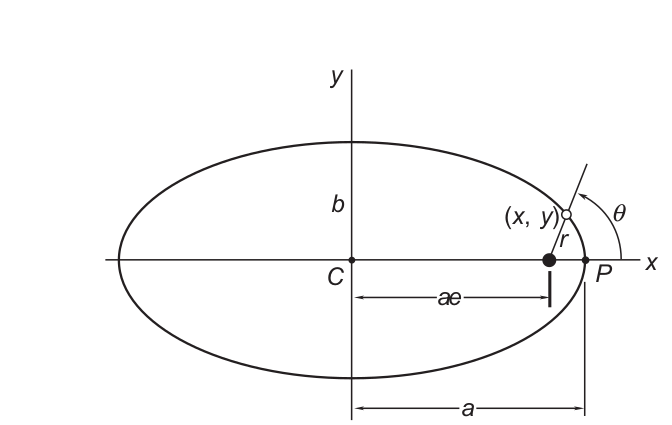
\includegraphics[width=\linewidth]{./Figures/ellipse_points.png}	
		\caption{Elementos de la elipse}
		\label{fig:elipse_pas}
	\end{subfigure}
	\hfill
	\begin{subfigure}[b]{0.49\linewidth}
		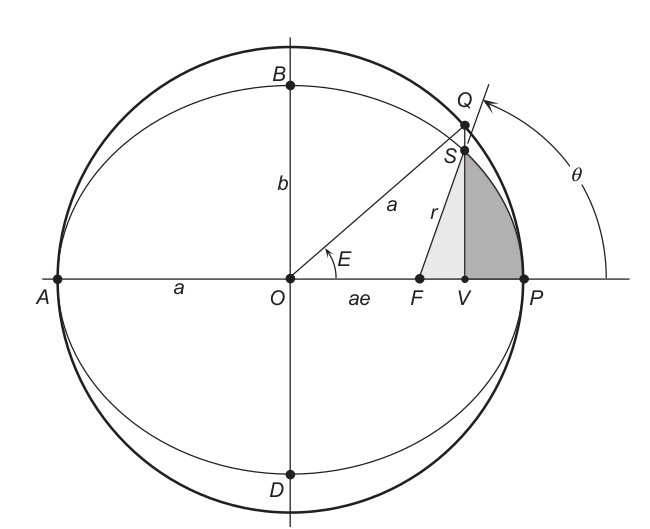
\includegraphics[width=\linewidth]{./Figures/ellipse_withE_time.png}
		\caption{Orbita en función del tiempo}
		\label{fig:ellipse_time}
	\end{subfigure}
	\caption{elementos de la elipse.}
	\label{fig:ellipse}
\end{figure}


siendo: 
\begin{itemize}
	\item $e$: excentricidad de la órbita
	\begin{itemize}
		\item $e = 0$: orbita circular
		\item $0<e <1$: orbita eliptica
		\item $e=1$: orbita parábolica
		\item $e>1$: orbita hiperbólica		
	\end{itemize}
	\item $\mu = G(M_{\oplus}+M_s) \approx G M_{\oplus} = 3.986 \times 10^{14} m^3/s^2 $: parametro gravitacional
	\item $h$:momento angular de la órbita
	\item $\theta$:anomalia verdadera
	\item $r$:posición del segundo cuerpo respecto del primero visto desde el foco
\end{itemize}

En este trabajo solo se trabaja con órbitas elipticas y circulares $0\leq e < 1$. La ecuación anterior, no brinda información sobre la evolución temporal de $\theta$. Para obtener esta información se define la anomalia media($M_e$), y el promedio de velocidad angular ($n$), el periodo de una órbita eliptica($T$, tiempo que tarda en recorrer un objeto un ángulo de 360° o 2$\pi $radianes) y la anomalia excentrica ($E$)(ver figura \ref{fig:ellipse_time}). Las relaciones entre ellos son(estas relaciones solo son validas en elipses y circulos, en el caso de un circulo se toma $e =0$ y $a$ como el radio del circulo):  
\begin{alignat}{3}
	T &= \frac{2\pi}{\sqrt{\mu}} a^{\frac{3}{2}} \\
	n &= 2\pi / T \\ 
	M_e &= nt \\
	M_e &= E-e\sin(E) \\
	\theta &= 2\arctan({  \sqrt{\frac{1-e}{1+e}}\tan(\frac{E}{2})})
\end{alignat}

Estas posición del vector $\vec{r}$ esta en un plano x-y. Para pasar de la órbita del plano, se definen otros tres elementos llamados
\begin{itemize}
	\item $\omega$ argumento del pergieo 
	\item $RAAN (\Omega)$: ascensión recta 
	\item $i$: inclinación  
\end{itemize}





\section{Dinámica y cinemática de un cuerpo rígido}



\section{Modelo de perturbaciones}
	\subsection{Gravity Gradient torq}
	\subsection{Magnetic Torq Field}
	

\section{Modelado de sensores}
\subsection{Sensor de Horizonte}
\subsection{Giroscopio}
\subsection{Magnetómetro}


\section{Control de actitud y señales de simulación}


\subsection{Actuador - Reaction Wheel}







